\documentclass{ctexart}
\usepackage{amsmath, mathrsfs, amsfonts}
\usepackage{tikz}
\usepackage{graphicx}
\usetikzlibrary{patterns}    % 绘制阴影区域需要加入的库

% library

\begin{document}

\begin{figure}[htp]
    \centering
    \begin{tikzpicture}[>=latex,scale=.7]
        \draw[->] (-5,0)--(5,0)node[right]{$x$};
        \draw[->] (0,-1)--(0,9)node[right]{$y$};
        \foreach \x in {-4,-2,2,4}
        {
            \draw (\x,0)node[below]{$\x$}--(\x,.1);
        }
        \foreach \y in {2,4,6,8}
        {
            \draw (0,\y)--node[left]{$\y$}(-.1,\y);
        }
        \foreach \x in {-3,-1,1,3}
        {
            \draw (\x,0)node[below]{$\x$}--(\x,.1);
        }
        \foreach \y in {1,3,5,7}
        {
            \draw (0,\y)--node[left]{$\y$}(-.1,\y);
        }
        \node at (-.25,-.25){$O$};

        \draw [domain=-4:4,samples=1000,thick] plot(\x,{0.5*\x*\x});    % domain -> 定义域,samples -> 采样点数
        \node at (4.5,6){$y=\dfrac{1}{2}x^2$};

        

    \end{tikzpicture}

    \caption{<caption>}
\end{figure}


\begin{figure}[htp]
    \centering
    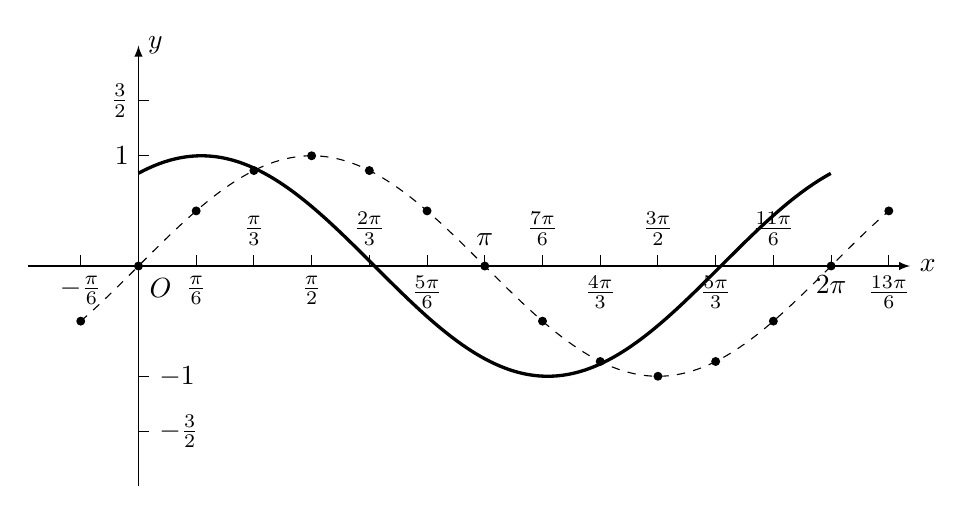
\begin{tikzpicture}[>=latex,scale=1.4]
        \draw[->] (-1,0)--(7,0)node[right]{$x$};
        \draw[->] (0,-2)--(0,2)node[right]{$y$};

        \draw [domain=-pi/6:13*pi/6,samples=1000,dashed] 
        plot(\x,{sin(\x r)});    % 角度和弧度之分,r -> 表示转换成弧度
        \draw [domain=0:2*pi,samples=1000,very thick] 
        plot(\x,{sin(\x r + 1 r)});    % y=sin(x+1)

        \draw (0,1)node[left]{1}--(0.1,1);
        \draw (0,1.5)node[left]{$\frac{3}{2}$}--(.1,1.5);
        \draw (0,-1)--(.1,-1)node[right]{$-1$};
        \draw (0,-1.5)--(.1,-1.5)node[right]{$-\frac{3}{2}$};

        \foreach \x/\xtext in {-1/-\frac{\pi}{6},1/\frac{\pi}{6},3/\frac{\pi}{2},
        5/\frac{5\pi}{6},8/\frac{4\pi}{3},10/\frac{5\pi}{3},12/2\pi,13/\frac{13\pi}{6}}
        {
            \draw (\x*pi/6,0)node[below]{$\xtext$}--(\x*pi/6,.1);
        }

        \foreach \x/\xtext in {2/\frac{\pi}{3},4/\frac{2\pi}{3},6/\pi,
        7/\frac{7\pi}{6},9/\frac{3\pi}{2},11/\frac{11\pi}{6}}
        {
            \draw (\x*pi/6,0)--(\x*pi/6,.1)node[above]{$\xtext$};
        }
        \node at (.2,-.2){$O$};
        
        \foreach \x in {-1,0,1,...,13}
        {
            \draw (\x*pi/6, {sin(\x*pi/6 r)}) [fill=black] circle (1pt);
        }




        

    \end{tikzpicture}

    \caption{<caption>}
\end{figure}



\end{document}